% CAPÍTULO 14 — a última volta: a janela e a lei que anda.
% Medição: lab/experimentos/E34_janela.ipynb. Figuras: figuras/E34_janela_1.pdf, E34_janela_3.pdf, E34_janela_2.pdf.
% Fracasso de abertura: a janela do corte e a memória de vinte e um dias foram medidas em mundos
% que não mudam ou que mudam de uma vez só; a porta que «ver mundos» deixou aberta — parâmetros
% que variam no tempo — nunca foi atravessada com instrumento na mão. Este capítulo atravessa.
% =============================================================================

\chapter{A janela certa quando a lei anda}
\label{cap:janela}

\section{A recomendação que nunca viu o mundo que anda}

Duas recomendações sustentam os instrumentos deste livro, e as duas nasceram em mundos que não
andam. A primeira é antiga: o corte mora numa janela de \numCorteJanela{} dias, decidida quando a
raiz aprendeu a medir. A segunda é mais recente: a memória de \numEsquecimentoMelhorMemoria{}
dias, a melhor que o capítulo da memória mede, e que ele mesmo delimita --- para a escala de um
mundo que dobra de uma vez, a janela de duzentos e cinquenta e dois dias erra por
\numEsquecimentoJanelaDuzentosECinquenta{} no começo, e o erro cai conforme a janela se renova,
porque o degrau acaba. O piso é o do mundo parado,
\numEsquecimentoPisoJanelaDuzentosECinquenta, e nenhuma janela pode prometer menos que ele. Até
aqui, mundo que muda de uma vez, ou mundo que não muda nunca.

O capítulo de ver mundos deixou uma porta declarada aberta, com nome na literatura: processos de
parâmetros que variam no tempo \cite{palma2010efficient} --- leis que andam devagar o bastante
para cada pedaço parecer parado \cite{dahlhaus1997estimation,dahlhaus2012locally}. A cauda convive com dias independentes de lei
pesada --- isso o capítulo da cauda mediu --- e sobrou a pergunta que este capítulo pega no bolso:
o que acontece com a janela quando a lei não muda de uma vez, mas anda? A deriva leve do capítulo
do orçamento já deu o preço de ver: memória de \numFormasMemoriaDerivaLeve{} dias, quatorze vezes
a janela do corte. O que não foi medido é o outro lado --- o que a lei que anda faz com a
estimativa que a persegue.

O fracasso pode ser declarado antes de qualquer número novo. Num mundo que anda, a janela não se
renova nunca: cada dia que passa ela atravessa uma lei diferente da que a calibrou, e não há
"depois da mudança" onde o erro volte ao piso. Se a recomendação de janela curta foi medida no
degrau, ela é uma recomendação sobre o degrau --- e dizer que vale para o mundo é afirmar mais do
que se mediu. A pergunta deste capítulo é se a medição separa os mundos: se a janela ótima se
move quando a forma do mundo muda, a recomendação única morre; se não se move, o mundo anda e a
janela nem fica sabendo.

\section{A varredura: onde o ótimo cai}

Quatro mundos, todos com a mesma oscilação de fundo, e a mudança declarada em cada forma: o mundo
parado, o degrau que dobra de uma vez, a rampa que dobra ao longo de um ano, e o mundo que anda
--- a rampa que nunca termina, com a escala crescendo a passo relativo constante, dobrando do
primeiro ao último dia. Em cada mundo, a mesma varredura: estimar a escala janela a janela, de
vinte e um a duas mil e dezesseis dias, e taxa a taxa, da memória de vinte e um dias à de mil e
oito, sempre contra a verdade declarada de cada dia, com o aquecimento pago por cada configuração
--- a avaliação começa no primeiro dia em que a estimativa existe depois da mudança.

\begin{figure}[t]
  \centering
  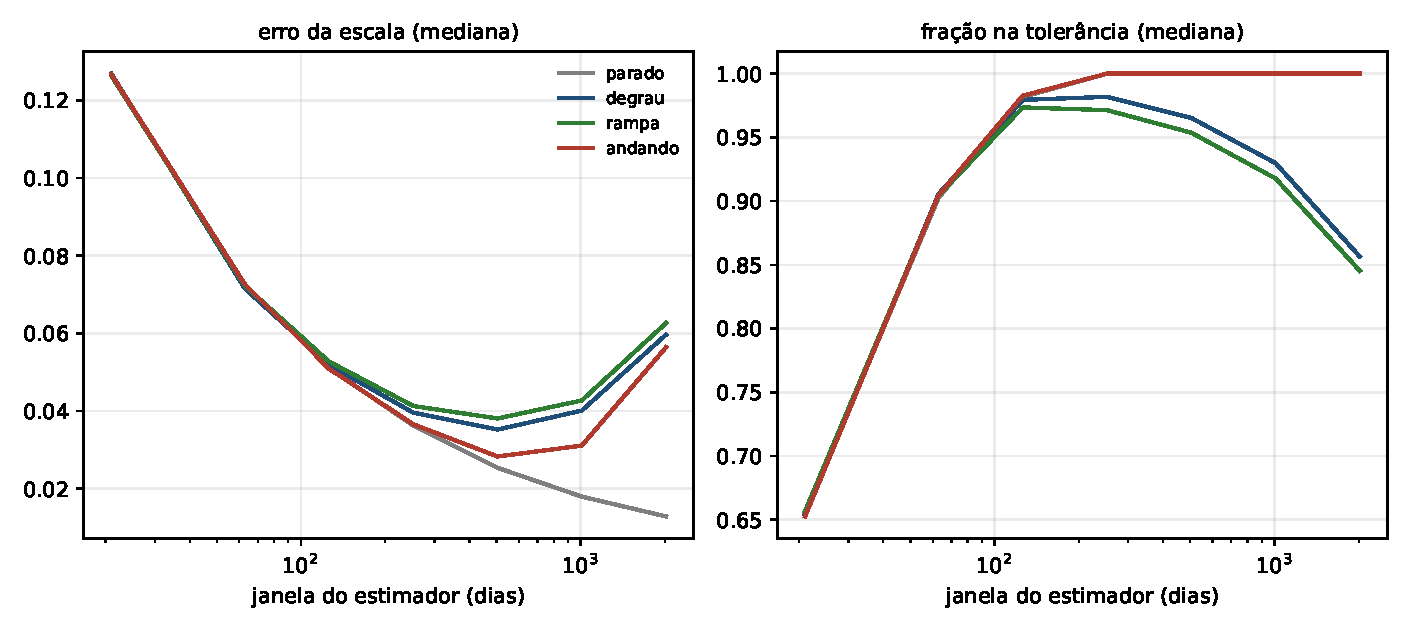
\includegraphics[width=\textwidth]{figuras/E34_janela_1.pdf}
  \caption{A varredura, forma por forma. À esquerda, o erro mediano da escala contra a janela do
    estimador: as formas que mudam fazem vale, com o fundo em quinhentos e quatro dias e subida de
    novo em seguida; o mundo parado desce sem virar. À direita, a fração de dias dentro da
    tolerância declarada: a tolerância não separa as formas --- quem separa é o erro.}
  \label{fig:janela:varredura}
\end{figure}

O ótimo se move, e é a medição central do capítulo. No mundo parado, a melhor janela é a maior
que foi tentada, \numJanelaParadoOtimoMediana{} dias, com a faixa entre mundos grudada nela ---
censura declarada: o ótimo verdadeiro está além, e mais janela só faria bem. Nas três formas que
mudam, o ótimo cai para \numJanelaDegrauOtimoMediana{} dias no degrau, \numJanelaRampaOtimoMediana{}
na rampa e \numJanelaAndandoOtimoMediana{} no mundo que anda, com as faixas apertadas em torno de
quinhentos e quatro. A memória conta a mesma história com outro número: a taxa vencedora guarda
\numJanelaParadoMemoriaVencedora{} dias no mundo parado e \numJanelaAndandoMemoriaVencedora{} no
mundo que anda.

O mecanismo é o atraso. A estimativa de uma janela é a média da lei dos últimos dias, e contra a
lei de hoje essa média chega atrasada; no mundo parado não há atraso nenhum a pagar, e mais janela
é só menos sorteio. No mundo que anda, cada dia a mais de janela compra menos sorteio e paga em
distância --- e o vale da curva é o ponto em que os dois preços se cruzam
\cite{dahlhaus1998optimal}. A janela de duas mil e dezesseis dias erra \numJanelaParadoErroDoisMilDezesseis{}
no mundo parado e \numJanelaAndandoErroDoisMilDezesseis{} no mundo que anda: quatro vezes mais.
A janela do corte, duzentos e cinquenta e dois dias, serve aos dois mal e por igual ---
\numJanelaParadoErroDuzentosCinquentaDois{} contra \numJanelaAndandoErroDuzentosCinquentaDois{}.
E a recomendação de janela curta do capítulo da memória? A janela de vinte e um dias erra
\numJanelaParadoErroVinteUm{} no mundo parado e \numJanelaAndandoErroVinteUm{} no que anda: em
patamar, e o pior de todos os tamanhos tentados nos dois mundos. A recomendação curta não é do
mundo que anda --- e a recomendação longa também não é.

Uma honestidade antes de seguir: a fração de dias dentro da tolerância declarada não separa forma
nenhuma --- em todas, a fração chega a \numJanelaParadoFracao{} a partir da janela do corte. A
tolerância é frouxa demais para ver o andar; quem vê é o erro. Instrumento que não distingue é
instrumento que promete pouco, e é bom saber qual dos dois é qual.

\section{A família que anda, ajustada}

A porta tem construção conhecida, e este capítulo a ajusta com o estimador mais simples que
existe, declarado: duas curvas por mercado, o coeficiente que puxa o retorno de hoje pelo de
ontem, janela a janela, e a escala de cada dia --- o desvio rolante, o instrumento do próprio
livro \cite{dahlhaus1997fitting}. O resultado do ajuste já é uma resposta: o coeficiente é quase
nada nos três mercados --- \numJanelaSpAGlobal{} no índice, \numJanelaIbovAGlobal{} no Ibovespa,
\numJanelaBtcAGlobal{} no Bitcoin --- e quem anda é a escala.

\begin{figure}[t]
  \centering
  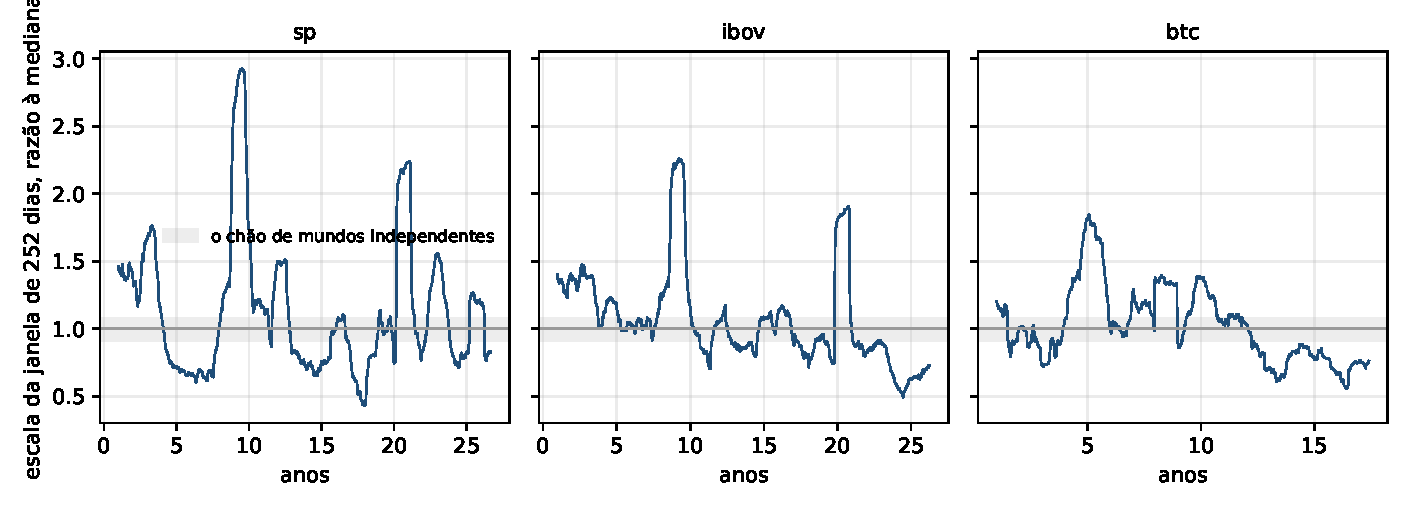
\includegraphics[width=\textwidth]{figuras/E34_janela_3.pdf}
  \caption{A lei que anda: a escala da janela de duzentos e cinquenta e dois dias, em razão à
    mediana de cada mercado, contra a banda do chão de mundos independentes (cinza). A escala
    caminha até perto de três vezes a mediana no índice e no Ibovespa, e até duas e meia no
    Bitcoin --- sempre muito além do chão.}
  \label{fig:janela:escala}
\end{figure}

Quanto a lei andou tem número, e o número tem chão. O orçamento da variação --- a soma dos passos
do logaritmo da escala, a moeda da casa para a medida que orça o movimento de parâmetros
\cite{chen2018stationary} --- dá \numJanelaSpOrcamento{} no índice, contra o chão de
\numJanelaSpOrcamentoChao{} que mundos independentes da mesma janela produzem; \numJanelaIbovOrcamento{}
contra \numJanelaIbovOrcamentoChao{} no Ibovespa, \numJanelaBtcOrcamento{} contra
\numJanelaBtcOrcamentoChao{} no Bitcoin. Em todos os três a lei andou acima do chão, e a distância
é o que a família ajustada carrega.

\section{A escada: quanto do pedaço é andar}

O capítulo do pedaço mediu a pergunta que falta responder: a entrega do corte, medida em pedaços
de dois anos, dispersa \numPedacoEntregaDispersaoDoisAnos{} entre pedaços, contra
\numPedacoEntregaIndependenteDoisAnos{} da conta de quem supõe dias independentes --- mais de
três vezes \cite{yu1994rates}. A diferença foi deixada como o preço de supor dias independentes.
A família que anda permite partir o preço em conta, com uma escada de três degraus: embaralhar os
dias do mercado, que destrói a dependência e o andar juntos; o ajuste de coeficiente fixo, que
guarda a dependência linear de média e mata o andar; e o ajuste que anda, as duas curvas do
capítulo. Cada degrau paga a mesma medição do pedaço.

\begin{table}[t]
  \centering
  \caption{A escada da dispersão entre pedaços de dois anos. Cada degrau é a mediana de
    \numJanelaReamostras{} reamostras; a coluna de referência é a dispersão medida do próprio
    mercado. O degrau do meio é plano: dependência linear de média não compra dispersão; o degrau
    que anda recupera quase toda no índice, metade no Ibovespa, pouco no Bitcoin --- e nenhum
    fecha a conta.}
  \label{tab:janela:escada}
  \resizebox{\linewidth}{!}{%
  \begin{tabular}{@{}lrrrr@{}}
    \hline
 & medido & embaralhado & coeficiente fixo & ajuste que anda \\
    \hline
índice & \numJanelaEscadaSpMedida{} & \numJanelaEscadaSpIndependente{} & \numJanelaEscadaSpAr{} & \numJanelaEscadaSpTvar{} \\
Ibovespa & \numJanelaEscadaIbovMedida{} & \numJanelaEscadaIbovIndependente{} & \numJanelaEscadaIbovAr{} & \numJanelaEscadaIbovTvar{} \\
Bitcoin & \numJanelaEscadaBtcMedida{} & \numJanelaEscadaBtcIndependente{} & \numJanelaEscadaBtcAr{} & \numJanelaEscadaBtcTvar{} \\
    \hline
  \end{tabular}}
\end{table}

\begin{figure}[t]
  \centering
  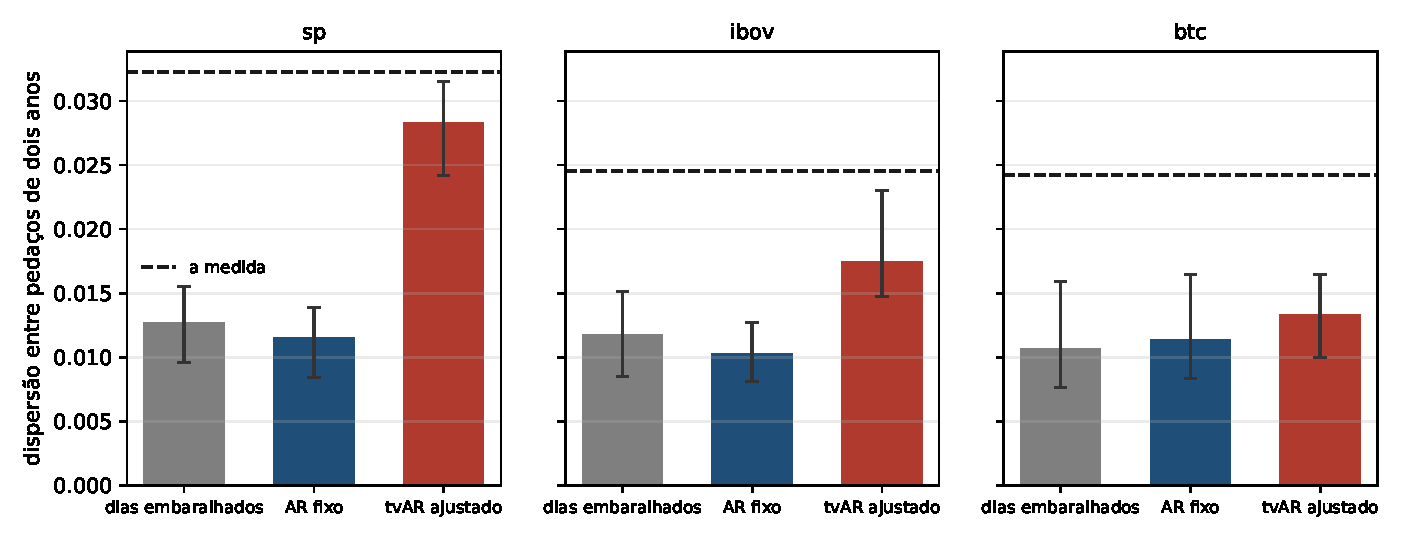
\includegraphics[width=\textwidth]{figuras/E34_janela_2.pdf}
  \caption{A escada da mesma tabela, em barras: a barra do ajuste que anda é a mais alta no índice
    e quase toca a linha da medida; no Ibovespa fica no meio do caminho; no Bitcoin as três ficam
    juntas e longe da linha. As barras são medianas de reamostras, com a faixa entre décimos.}
  \label{fig:janela:escada}
\end{figure}

A leitura é em dois tempos, e o primeiro é uma declaração de falha: o critério que este capítulo
declarou --- cada degrau aproximar a medida mais que o anterior --- não se cumpre, porque o degrau
do meio é plano. Embaralhar os dias e ajustar o coeficiente fixo dão o mesmo pé nos três
mercados. E a falha é a informação: a dependência linear de média, que era a suspeita herdada do
capítulo do pedaço, não compra nada da dispersão. O segundo tempo é o degrau que anda: ele sobe
sozinho, e sobe em gradiente. No índice, \numJanelaEscadaSpTvar{} contra \numJanelaEscadaSpMedida{}
medidos --- quase toda a conta. No Ibovespa, \numJanelaEscadaIbovTvar{} contra
\numJanelaEscadaIbovMedida{}: metade do caminho. No Bitcoin, \numJanelaEscadaBtcTvar{} contra
\numJanelaEscadaBtcMedida{}: pouco. E em nenhum dos três a conta fecha --- o que sobra não é
dependência de média nem a lei que anda da escala; é outra coisa, e o livro ainda a carrega.

\section{A região: a porta não é a conta da geometria}

Falta a pergunta que fecha a porta por dentro: a família que anda explica a geometria? O método
é o do capítulo da tolerância: contar quantos membros da família reproduzem as quatro estatísticas
do dado dentro da tolerância da casa. Os membros são as janelas das curvas e a lei do sorteio ---
gaussiana ou de cauda pesada ---, oito no total, cada um simulado \numJanelaMundosRegiao{} vezes.

Nenhum reproduz. Zero de \numJanelaRegiaoSpTentados{} no índice, zero no Ibovespa, zero no
Bitcoin --- a melhor folga é \numJanelaRegiaoSpFolgaSessentaTresNormal{} no índice,
\numJanelaRegiaoIbovFolgaSessentaTresNormal{} no Ibovespa e
\numJanelaRegiaoBtcFolgaSessentaTresNormal{} no Bitcoin, sempre no membro de janela mais curta, e
a cauda pesada só piora a folga. A família que anda explica o andar da escala e parte da
dispersão entre pedaços, e não reproduz a geometria: as duas explicações que sobraram no capítulo
da geometria continuam de pé, agora com a porta medida e não apenas declarada. Ver mundos não
basta --- e atravessar a porta também não é chegada.

\section{O que fica}

A resposta à pergunta do título é que a pergunta estava mal feita. Não existe a janela certa;
existe a janela certa de cada mundo, e ela se move quando o mundo muda de forma: censurada no
tamanho maior tentado no mundo parado, em quinhentos e quatro dias nas formas que mudam, com a
memória vencedora caindo de \numJanelaParadoMemoriaVencedora{} para
\numJanelaAndandoMemoriaVencedora{} dias quando a lei anda. Toda recomendação de janela é uma
afirmação sobre o mundo em que foi medida --- e a recomendação de janela curta deste livro é,
medida a terra em volta, uma recomendação sobre o degrau.

A porta que o capítulo de ver mundos deixou aberta foi atravessada com instrumento na mão, e o
que havia do outro lado foi medido: uma escala que anda muito além do chão independente nos três
mercados, um orçamento de variação acima do chão em todos, quase toda a dispersão entre pedaços do
índice explicada pelo andar --- e nenhuma reprodução da geometria. A família mais rica não derruba
o que o livro construiu; ela soma uma conta, e a conta tem gradiente entre mercados que nenhuma
unificação declarada cobre.

O que sobra é a intervenção, e com ela o fracasso seguinte. Não basta querer intervir: é preciso
dizer que intervenção distinguiria as duas famílias de explicação que a mesma série admite, e
quanto ela custaria em dado que não existe. Um experimento que não se pode fazer é uma opinião com
instrumentos; um que se pode fazer é uma medida, e é essa diferença que a travessia ainda tem de
enfrentar.
